\chapter{AMQP Workflow Orchestration}\label{sec:amqp-workflow-orch}



\section{Overview}

A message queue that supports the AMQP protocol is used to maintain state for \cxoneflow
workflows.  The schema for the exchanges and queues is depicted in Figure \ref{fig:amqp-schema}.
The \texttt{Scan In} exchange is the entrypoint for all workflow state messages.  It is possible
to bind custom topic exchanges and create custom queues to augment or replace some of the
workflows.


\begin{figure}[h]
    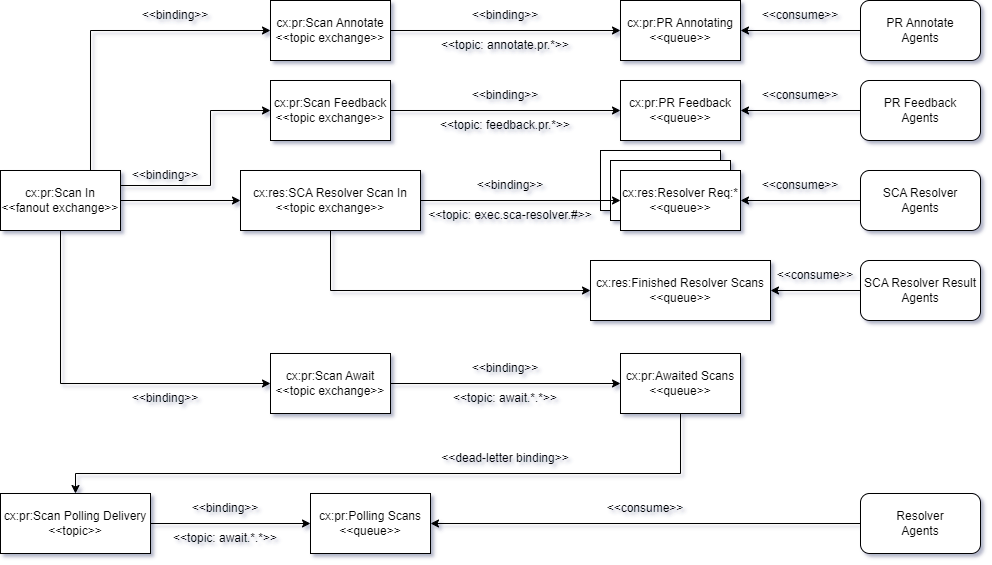
\includegraphics[width=\textwidth]{graphics/cxoneflow-diagrams-Queue.png}
    \caption{AMQP Schema for \cxoneflow}
    \label{fig:amqp-schema}
\end{figure}


Upon startup, each \cxoneflow instance will configure the exchange/queue schema.  An
internal instance of RabbitMQ runs inside the \cxoneflow container to orchestrate
workflows for the container instance.  If an AMQP connection configuration, described in
Section \ref{sec:yaml-config}, is not provided then the local RabbitMQ instance is
used.  When the container is exited, all persisted workflow state information in the local
RabbitMQ instance is lost.  To persist workflow state across container restarts, please
refer to Appendix \ref{sec:high-availability} to deploy \cxoneflow in a
high-availability configuration.

